\begin{figure*}[]
    \centering
    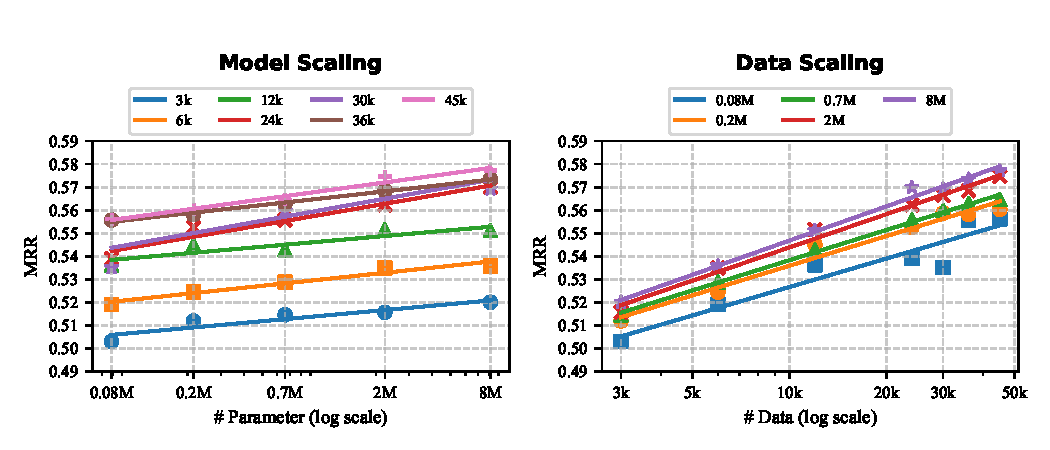
\includegraphics[width=5.5in]{images/scaling_separate.pdf}
    % \vspace{-.6cm}
    \caption{The illustration of the model and data scaling law of \ourmethod.}
    \label{fig:scaling_separate}
    % \vspace{-0.5cm}
\end{figure*}


    \begin{table}[]
\centering
\caption{The different number of layers with corresponding model size and performance for scaling law analysis.}
\label{tab:layers}
% \resizebox{\columnwidth}{!}{%
\begin{tabular}{@{}c|cc|cc|cc|cc@{}}
    \toprule
Hidden Dim. = 512     & \multicolumn{2}{c|}{Averge}   & \multicolumn{2}{c|}{HotpotQA} & \multicolumn{2}{c|}{MuSiQue}  & \multicolumn{2}{c}{2Wiki}     \\ \midrule
L-Layer       & R@2           & R@5           & R@2           & R@5           & R@2           & R@5           & R@2           & R@5           \\ \midrule
1-layer (3M)  & 53.9          & 66.7          & 59.3          & 74.2          & 40.7          & 50.2          & 61.8          & 75.7          \\
2-layer (4M)  & 69.9          & 78.6          & 73.6          & 85.4          & 47.6          & 57.0          & 88.6          & 93.3          \\
4-layer (6M)  & 72.2          & \textbf{80.1} & 78.4          & 87.8          & 49.3          & \textbf{60.1} & 88.8          & 92.5          \\
6-layer (8M)  & 71.9          & 79.6          & 78.0          & 87.0          & 48.4          & 58.7          & 89.3          & 93.1          \\
8-layer (10M) & \textbf{73.0} & 79.9          & \textbf{79.7} & \textbf{87.8} & \textbf{49.7} & 59.1          & \textbf{89.5} & \textbf{92.8}\\ \bottomrule
\end{tabular}%
% }
\end{table}